\label{sec:peer_joining}
\begin{figure*}
  %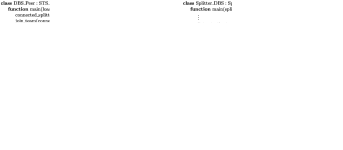
\includegraphics[width=\textwidth]{joining}
  \fig{700}{7cm}{joining} \caption{Procedures involved in a peer
    joining.\label{fig:joining}}
\end{figure*}

As can be seen in Fig.~\ref{fig:joining}, incoming peers request
(using a reliable\footnote{Reliable messages are transmitted over TCP
and their transmission is denoted in the pseudocode by
$\Rightarrow$. On the other hand, unreliable messages, which can be
lost in transit, are transmitted over UDP and its transmission is
denoted by $\rightarrow$. In any case, the reception of a packet is a
permanent blocking action, at least a timeout is indicated.}
communication) to the splitter the current list of peers in the
team. To minimize the joining time, a $[\mathtt{hello}]$ message is
sent to each peer of the team in parallel with the reception of the
list. When a peer of the team receives a $[\mathtt{hello}]$, it runs
the $\mathrm{add}\_\mathrm{neighbor}()$ function, which basically: (1)
adds the sender of the message to a table of peers called
$\mathrm{forward}[]$ (if in peer $P_i$ there is an entry
$\mathrm{forward}[P_j]=P_k$ then, each chunk received by $P_i$ and
originated at $P_j$ will be forwarded to $P_k$), initializes the table
$\mathrm{debt}[]$ (which stores the chunk debts between neighbor
peers), and (3) sets the variable $\mathrm{neighbor}$ with an index to
$\mathrm{forward}[]$ (see Sec.~\ref{sec:chunk_DBS_processing}).
